\documentclass[11pt]{article}

\usepackage[margin=0.75in]{geometry}
\usepackage[table]{xcolor}
\usepackage{booktabs}
\usepackage{graphicx}
\usepackage{multirow}
\usepackage{float}

\newcommand{\na}{--}
\newcommand{\notcalc}{not calc.}
\newcommand{\repro}{Reproduce}
\newcommand{\vidcom}{VidCom$^2$}

\title{Main Experiment Tables with Local Reproduction Rows}
\author{Reproduction summary}
\date{}

\begin{document}
\maketitle

\section{PruneVid}

\begin{table}[H]
\centering
\scriptsize
\resizebox{\textwidth}{!}{%
\begin{tabular}{lccccc}
\toprule
\textbf{Method} & \textbf{Retained} & \textbf{FLOPs} & \textbf{MVBench} & \textbf{VideoMME} & \textbf{EgoSchema (Subset / Fullset)} \\
\midrule
PLLaVA & 100.0\% & 1.00$\times$ & 46.6 & 44.4 & 47.8 / 42.6 \\
PLLaVA w/ FastV & 30.0\% & 0.33$\times$ & 46.1 & 43.6 & 46.2 / 41.0 \\
PLLaVA w/ Prumerge & 55.7\% & 0.53$\times$ & 45.6 & 43.8 & 45.2 / 40.4 \\
PLLaVA w/ Look-M & 20.0\% & 1.00$\times$ & 46.6 & 44.3 & 47.0 / 42.3 \\
\rowcolor{blue!8}
PLLaVA w/ Ours & \textbf{16.2\%} & \textbf{0.23$\times$} & \textbf{47.6} & \textbf{45.0} & \textbf{49.0} / \textbf{42.6} \\
\rowcolor{green!8}
PLLaVA w/ Ours (\repro) & 16.2\% & 0.23$\times$ & 46.42 & 44.89 & 48.40 / 41.90 \\
\midrule
ST-LLM & 100.0\% & 1.00$\times$ & 54.9 & 42.0 & 56.2 / 45.6 \\
ST-LLM w/ FastV & 30.0\% & 0.37$\times$ & 42.9 & 34.5 & 48.0 / 38.5 \\
ST-LLM w/ Look-M & 20.0\% & 1.00$\times$ & 54.0 & 40.6 & 54.0 / 44.5 \\
\rowcolor{blue!8}
ST-LLM w/ Ours & \textbf{15.1\%} & \textbf{0.26$\times$} & \textbf{54.3} & \textbf{41.4} & \textbf{54.6} / \textbf{44.7} \\
\rowcolor{green!8}
ST-LLM w/ Ours (\repro, self-port) & 15.1\% & 0.26$\times$ & 54.80 & 42.59 & 59.80 / 45.10 \\
\midrule
LLaVA-OneVision & 100.0\% & 1.00$\times$ & 58.0 & 58.2 & 62.0 / 60.0 \\
LLaVA-OneVision w/ FastV & 30.0\% & 0.30$\times$ & 57.2 & 57.6 & 62.6 / 60.0 \\
LLaVA-OneVision w/ Prumerge & 55.2\% & 0.49$\times$ & 52.9 & 56.7 & 62.2 / 60.0 \\
LLaVA-OneVision w/ Look-M & 20.0\% & 1.00$\times$ & 57.0 & 58.0 & 62.0 / \textbf{59.8} \\
\rowcolor{blue!8}
LLaVA-OneVision w/ Ours & \textbf{17.0\%} & \textbf{0.20$\times$} & \textbf{57.5} & \textbf{58.6} & \textbf{62.6} / 59.5 \\
\rowcolor{green!8}
LLaVA-OneVision w/ Ours (\repro, self-port) & 17.0\% & 0.20$\times$ & 57.23 & 58.37 & 64.40 / 61.78 \\
\bottomrule
\end{tabular}}
\caption{PruneVid main experiment table with local reproduction rows inserted below the paper Ours rows. PLLaVA uses the released implementation; ST-LLM and LLaVA-OneVision are self-ported because the official repository marks those PruneVid backbones as not yet released.}
\label{tab:prunevid-main}
\end{table}

\begin{figure}[H]
\centering
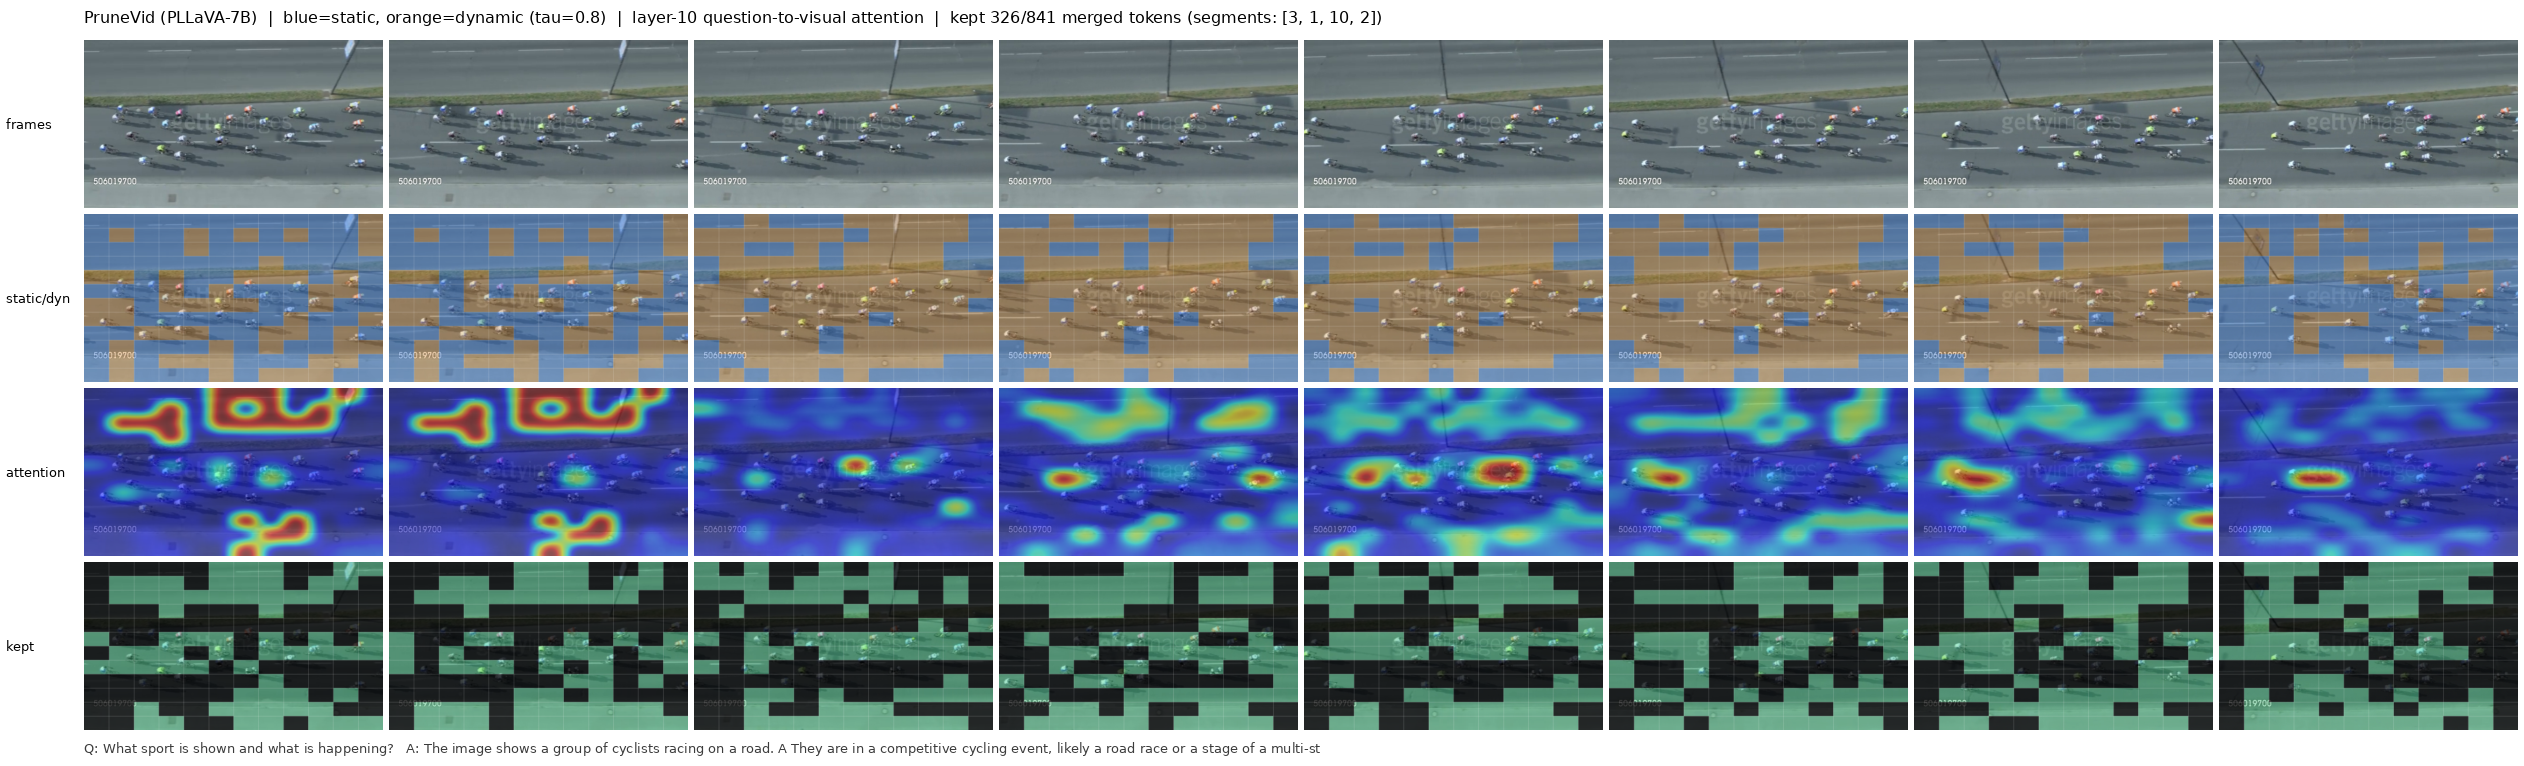
\includegraphics[width=\textwidth]{visualizations/out/prunevid_cycling_race.png}
\caption{Qualitative visualization of PruneVid's stages on a new cycling-race video (PLLaVA-7B, 16 frames, $12\times12$ grid), captured from the same instrumented code path as the table above. Row 2: static (\textcolor[RGB]{70,130,220}{blue}) vs.\ dynamic (\textcolor[RGB]{220,120,0}{orange}) patches ($\tau=0.8$) --- the moving peloton is dynamic while road and background are static and merged temporally. Row 3: layer-10 question-to-visual attention broadcast back to patches (smoothed, as in the paper). Row 4: tokens kept by the LLM-stage top-$\alpha$ selection ($\alpha=0.4$), which tracks the cyclists. More examples in \texttt{visualizations/out/}.}
\end{figure}

\begin{figure}[H]
\centering
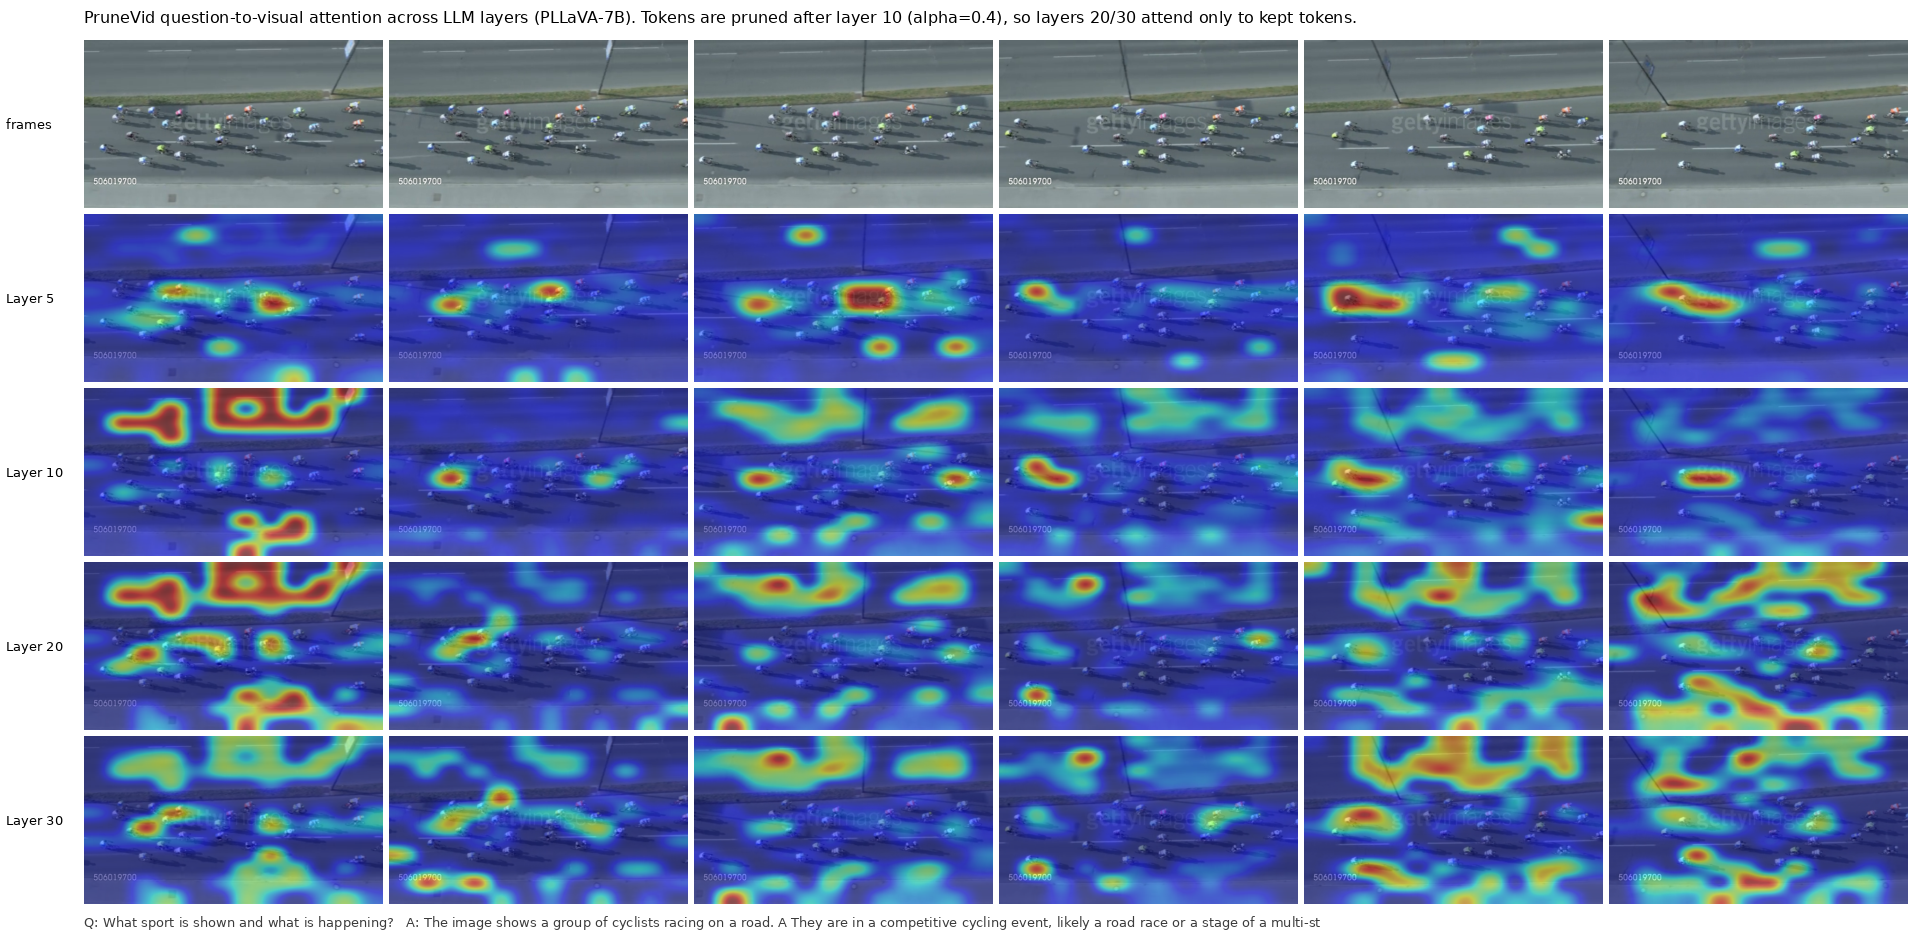
\includegraphics[width=\textwidth]{visualizations/out/prunevid_attn_layers_cycling_race.png}
\caption{Question-to-visual attention across LLM layers on the same video, mirroring the attention-evolution visualization in the PruneVid paper (Fig.~1c). Attention is max-pooled over heads and question tokens, broadcast back to patches through the merge metadata, and rendered as smoothed heatmaps. Tokens are pruned after layer 10 ($\alpha=0.4$), so layers 20/30 attend only to the kept tokens; attention progressively concentrates on the question-relevant regions (the peloton).}
\end{figure}

\section{VidCom$^2$}

\begin{table}[H]
\centering
\scriptsize
\resizebox{\textwidth}{!}{%
\begin{tabular}{llcccccccc}
\toprule
\textbf{Backbone} & \textbf{Method / Ratio} & \textbf{MVBench} & \textbf{LongVideoBench} & \textbf{MLVU} & \textbf{VideoMME} & \textbf{Short} & \textbf{Medium} & \textbf{Long} & \textbf{Average (\%)} \\
\midrule
LLaVA-OV-7B & Upper bound & 56.9 & 56.4 & 63.0 & 58.6 & 70.3 & 56.6 & 48.8 & 100.0 \\
LLaVA-OV-7B & DyCoke, $R=30\%$ & 56.6 & 54.7 & 60.3 & 56.1 & 67.1 & 54.6 & 46.6 & 96.5 \\
LLaVA-OV-7B & Random, $R=25\%$ & 54.2 & 52.7 & 59.7 & 55.6 & 65.4 & 53.0 & 48.3 & 94.8 \\
LLaVA-OV-7B & FastV, $R=25\%$ & 55.5 & 53.3 & 59.6 & 55.3 & 65.0 & 53.8 & 47.0 & 94.9 \\
LLaVA-OV-7B & PDrop, $R=25\%$ & 55.3 & 51.3 & 57.1 & 55.5 & 64.7 & 53.1 & 48.7 & 94.1 \\
LLaVA-OV-7B & SparseVLM, $R=25\%$ & 56.4 & 53.9 & 60.7 & 57.3 & 68.4 & 55.2 & 48.1 & 97.5 \\
LLaVA-OV-7B & DyCoke, $R=25\%$ & 49.5 & 48.1 & 55.8 & 51.0 & 61.1 & 48.6 & 43.2 & 87.0 \\
\rowcolor{blue!8}
LLaVA-OV-7B & \textbf{VidCom$^2$, $R=25\%$} & \textbf{57.2} & \textbf{54.9} & \textbf{62.5} & \textbf{58.6} & \textbf{69.8} & \textbf{56.4} & \textbf{49.4} & \textbf{99.6} \\
\rowcolor{green!8}
LLaVA-OV-7B & VidCom$^2$, $R=25\%$ (\repro) & 57.00 & 55.27 & 62.09 & 58.33 & 69.33 & 56.56 & 49.11 & 99.3 \\
LLaVA-OV-7B & FastV, $R=15\%$ & 51.6 & 48.3 & 55.0 & 48.1 & 51.4 & 49.4 & 43.3 & 85.0 \\
LLaVA-OV-7B & PDrop, $R=15\%$ & 53.2 & 47.6 & 54.7 & 50.1 & 58.7 & 48.7 & 45.0 & 87.4 \\
LLaVA-OV-7B & SparseVLM, $R=15\%$ & 52.9 & 49.7 & 57.4 & 53.4 & 61.0 & 52.1 & 47.0 & 91.2 \\
\rowcolor{blue!8}
LLaVA-OV-7B & \textbf{VidCom$^2$, $R=15\%$} & \textbf{54.3} & \textbf{52.0} & \textbf{58.9} & \textbf{56.2} & \textbf{65.8} & \textbf{54.8} & \textbf{48.1} & \textbf{95.1} \\
\rowcolor{green!8}
LLaVA-OV-7B & VidCom$^2$, $R=15\%$ (\repro) & 54.48 & 53.10 & 60.47 & 55.74 & 65.56 & 53.78 & 47.89 & 95.2 \\
\midrule
LLaVA-Video-7B & Upper bound & 60.4 & 59.6 & 70.3 & 64.3 & 77.2 & 62.1 & 53.4 & 100.0 \\
LLaVA-Video-7B & DyCoke, $R=30\%$ & 57.5 & 55.5 & 60.6 & 61.3 & 73.4 & 59.3 & 51.2 & 93.8 \\
LLaVA-Video-7B & FastV, $R=25\%$ & 53.8 & 51.2 & 57.8 & 59.3 & 67.1 & 60.0 & \textbf{50.8} & 89.7 \\
LLaVA-Video-7B & SparseVLM, $R=25\%$ & 55.4 & 54.2 & 58.9 & 60.1 & 71.1 & 59.1 & 50.1 & 91.6 \\
LLaVA-Video-7B & DyCoke, $R=25\%$ & 50.8 & 53.0 & 56.9 & 56.1 & 65.8 & 53.6 & 48.9 & 86.3 \\
\rowcolor{blue!8}
LLaVA-Video-7B & \textbf{VidCom$^2$, $R=25\%$} & \textbf{57.0} & \textbf{55.5} & \textbf{59.0} & \textbf{61.7} & \textbf{73.0} & \textbf{61.7} & 50.0 & \textbf{93.6} \\
\rowcolor{green!8}
LLaVA-Video-7B & VidCom$^2$, $R=25\%$ (\repro) & 56.88 & 56.62 & 57.24 & 61.85 & 72.89 & 61.67 & 51.00 & 93.5 \\
LLaVA-Video-7B & FastV, $R=15\%$ & 44.0 & 44.6 & 53.8 & 51.3 & 56.4 & 51.1 & 46.2 & 78.0 \\
LLaVA-Video-7B & SparseVLM, $R=15\%$ & 53.1 & \textbf{52.7} & 56.2 & 55.7 & 65.0 & 53.9 & 48.3 & 86.3 \\
\rowcolor{blue!8}
LLaVA-Video-7B & \textbf{VidCom$^2$, $R=15\%$} & \textbf{53.3} & 51.5 & \textbf{56.8} & \textbf{58.3} & \textbf{68.0} & \textbf{57.3} & \textbf{49.7} & \textbf{88.5} \\
\rowcolor{green!8}
LLaVA-Video-7B & VidCom$^2$, $R=15\%$ (\repro) & 53.33 & 52.28 & 54.94 & 58.22 & 68.00 & 56.89 & 49.78 & 88.0 \\
\bottomrule
\end{tabular}}
\caption{VidCom$^2$ main experiment table with local LLaVA-OV and LLaVA-Video reproduction rows inserted below the corresponding paper rows. Average(\%) follows the paper's convention: the row's 7-column sum (MVBench, LongVideoBench, MLVU, VideoMME, Short/Medium/Long) divided by the corresponding Upper-bound row's 7-column sum. Reproduced Average(\%) matches the paper within $\le0.5$ pts on all four rows (OV $R{=}25\%$: 99.3 vs 99.6; OV $R{=}15\%$: 95.2 vs 95.1; Video $R{=}25\%$: 93.5 vs 93.6; Video $R{=}15\%$: 88.0 vs 88.5).}
\label{tab:vidcom-main}
\end{table}

\begin{figure}[H]
\centering
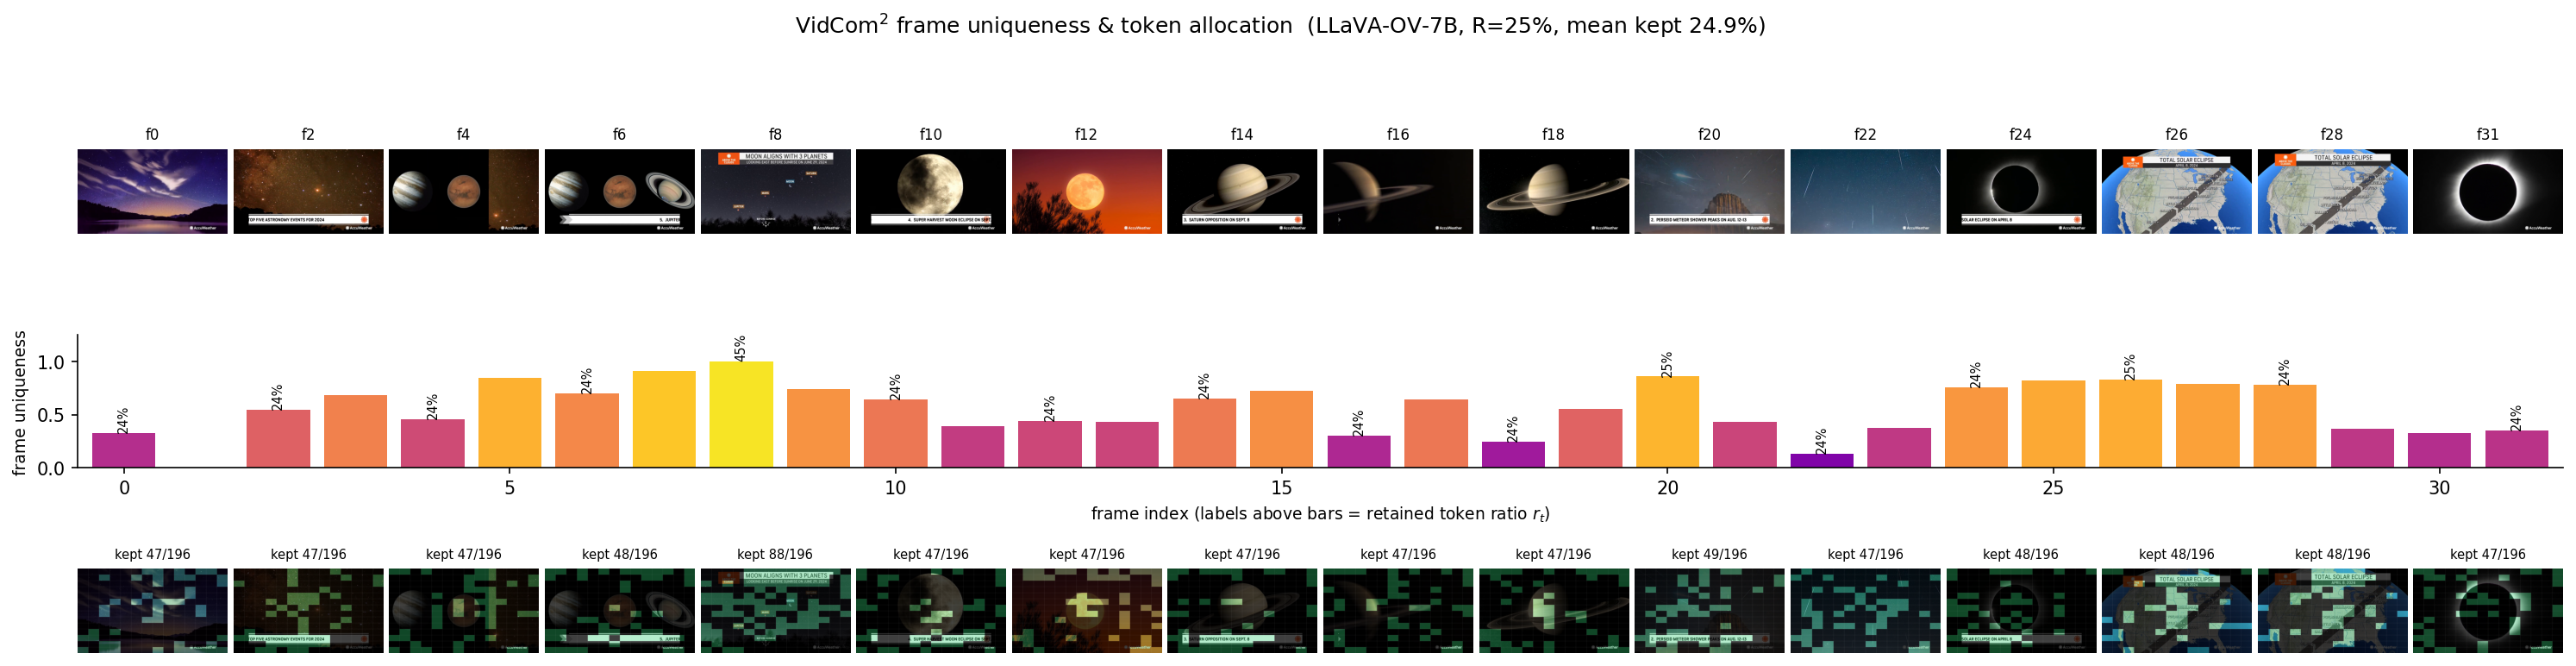
\includegraphics[width=\textwidth]{visualizations/out/vidcom2_uniqueness_videomme_08km9Yqbt.png}
\caption{Qualitative visualization of VidCom$^2$ frame uniqueness and token allocation on a new Video-MME astronomy video (LLaVA-OV-7B, $R=25\%$). Taller/brighter bars mark more unique frames, which receive a larger per-frame retention ratio $r_t$ (labels above bars); visually redundant frames are compressed harder. Bottom: the retained $14\times14$ patches per frame. More examples in \texttt{visualizations/out/}.}
\end{figure}

\section{AOT}

\begin{table}[H]
\centering
\scriptsize
\resizebox{\textwidth}{!}{%
\begin{tabular}{lccc|cccc|cc}
\toprule
\textbf{Method} & \textbf{Prefill FLOPs} & \textbf{FLOPs Ratio} & \textbf{Retained} & \textbf{MVBench} & \textbf{EgoSchema} & \textbf{LongVideoBench} & \textbf{VideoMME} & \textbf{Avg. Score} & \textbf{Avg. \%} \\
\midrule
LLaVA-OV-7B & 40.8 & 100\% & 100\% & 58.3 & 60.4 & 56.4 & 58.6 & 58.4 & 100.0 \\
FastV & 9.3 & 22.8\% & 100\% & 55.9 & 57.5 & \textbf{56.7} & 56.1 & 56.5 & 96.7 \\
PDrop & 10.5 & 25.7\% & 100\% & 56.1 & 58.0 & 54.1 & 56.4 & 56.2 & 96.2 \\
DyCoke & 8.7 & 21.3\% & 25\% & 53.1 & 59.5 & 49.5 & 54.3 & 54.1 & 92.6 \\
VisionZip & 8.7 & 21.3\% & 25\% & 57.9 & 60.3 & 56.5 & 58.2 & 58.2 & 99.7 \\
PruneVid & 8.7 & 21.3\% & 25\% & 57.4 & 59.9 & 55.7 & 57.4 & 57.6 & 98.6 \\
FastVID & 8.7 & 21.3\% & 25\% & 56.5 & \na & 56.3 & 58.0 & \na & \na \\
\rowcolor{blue!8}
\textbf{AOT} & 8.7 & 21.3\% & 25\% & \textbf{58.7} & \textbf{61.3} & 56.3 & 57.5 & \textbf{58.5} & \textbf{100.0} \\
\rowcolor{green!8}
AOT (\repro) & 8.7 & 21.3\% & 25\% & 57.75 & 61.18 & 54.75 & 54.89 & 57.14 & 97.8 \\
VisionZip & 7.0 & 17.2\% & 20\% & 57.7 & 59.8 & 55.2 & 57.9 & 57.7 & 98.8 \\
PruneVid & 7.0 & 17.2\% & 20\% & 57.2 & 59.7 & 54.7 & 56.9 & 57.1 & 97.8 \\
FastVID & 7.0 & 17.2\% & 20\% & 56.3 & \na & \textbf{57.1} & \textbf{57.9} & \na & \na \\
\rowcolor{blue!8}
\textbf{AOT} & 7.0 & 17.2\% & 20\% & \textbf{58.1} & \textbf{61.3} & 56.2 & 57.2 & \textbf{58.2} & \textbf{99.7} \\
\rowcolor{green!8}
AOT (\repro) & 7.0 & 17.2\% & 20\% & 57.73 & 61.22 & 54.08 & 54.78 & 56.95 & 97.5 \\
VisionZip & 5.2 & 12.7\% & 15\% & 56.5 & 59.8 & 54.4 & 56.1 & 56.7 & 97.1 \\
PruneVid & 5.2 & 12.7\% & 15\% & 56.8 & 59.7 & 55.4 & 56.6 & 57.1 & 97.8 \\
FastVID & 5.2 & 12.7\% & 15\% & 56.0 & \na & \textbf{56.2} & \textbf{57.7} & \na & \na \\
\rowcolor{blue!8}
\textbf{AOT} & 3.4 & 8.3\% & 15\% & \textbf{57.8} & \textbf{61.3} & 55.2 & 56.6 & \textbf{57.7} & \textbf{98.8} \\
\rowcolor{green!8}
AOT (\repro) & 3.4 & 8.3\% & 15\% & 57.33 & 60.98 & 52.80 & 54.22 & 56.33 & 96.5 \\
VisionZip & 3.4 & 8.3\% & 10\% & 53.5 & 58.0 & 49.3 & 53.4 & 53.5 & 91.6 \\
PruneVid & 3.4 & 8.3\% & 10\% & 56.2 & 59.8 & 54.5 & 56.0 & 56.6 & 96.9 \\
FastVID & 3.4 & 8.3\% & 10\% & 55.9 & \na & \textbf{56.3} & \textbf{57.3} & \na & \na \\
\rowcolor{blue!8}
\textbf{AOT} & 5.2 & 12.7\% & 10\% & \textbf{57.0} & \textbf{60.6} & 54.2 & 56.1 & \textbf{57.0} & \textbf{97.6} \\
\rowcolor{green!8}
AOT (\repro) & 5.2 & 12.7\% & 10\% & 56.70 & 60.45 & 52.65 & 53.78 & 55.90 & 95.7 \\
\bottomrule
\end{tabular}}
\caption{AOT main experiment table on LLaVA-OneVision with local reproduction rows inserted below the corresponding paper AOT rows. All runs follow the authors' released evaluation config (\texttt{eval\_ov-7b.sh}); EgoSchema full-test accuracy is obtained by submitting local predictions to the official validation server; LongVideoBench and VideoMME use a VTN-calibrated sweep so measured token retention matches the labeled ratios. Averages are computed over the four benchmarks, with Avg.\ \% relative to the full-model baseline.}
\label{tab:aot-ov-main}
\end{table}

\begin{table}[H]
\centering
\scriptsize
\resizebox{\textwidth}{!}{%
\begin{tabular}{lccc|cccc|cc}
\toprule
\textbf{Method} & \textbf{Prefill FLOPs} & \textbf{FLOPs Ratio} & \textbf{Retained} & \textbf{MVBench} & \textbf{EgoSchema} & \textbf{LongVideoBench} & \textbf{VideoMME} & \textbf{Avg. Score} & \textbf{Avg. \%} \\
\midrule
LLaVA-Video-7B & 80.2 & 100\% & 100\% & 60.4 & 57.2 & 58.9 & 64.3 & 60.2 & 100.0 \\
FastV & 17.1 & 21.3\% & 100\% & 54.3 & 54.1 & 55.0 & 58.8 & 55.6 & 92.4 \\
PDrop & 19.5 & 24.3\% & 100\% & 55.9 & 54.3 & 54.7 & 61.9 & 56.7 & 94.2 \\
VisionZip & 9.3 & 18.9\% & 25\% & 56.7 & 54.7 & 54.7 & 60.7 & 56.7 & 94.2 \\
DyCoke & 9.3 & 18.9\% & 25\% & 50.8 & \na & 53.0 & 56.9 & \na & \na \\
\rowcolor{blue!8}
\textbf{AOT} & 9.3 & 18.9\% & 25\% & \textbf{58.8} & \textbf{55.4} & \textbf{56.2} & \textbf{62.4} & \textbf{58.2} & \textbf{96.7} \\
\rowcolor{green!8}
AOT (\repro) & 9.3 & 18.9\% & 25\% & 58.42 & 55.85$^\ddagger$ & 56.24 & 62.52 & 58.26 & 96.8 \\
VisionZip & 9.3 & 11.6\% & 15\% & 56.7 & 54.7 & 54.7 & 60.7 & 56.7 & 94.2 \\
\rowcolor{blue!8}
\textbf{AOT} & 9.3 & 11.6\% & 15\% & \textbf{57.8} & \textbf{55.2} & \textbf{55.0} & \textbf{62.0} & \textbf{57.5} & \textbf{95.5} \\
\rowcolor{green!8}
AOT (\repro) & 9.3 & 11.6\% & 15\% & 57.98 & 55.08$^\ddagger$ & 55.42 & 62.11 & 57.65 & 95.8 \\
\bottomrule
\end{tabular}}
\caption{AOT main experiment table on LLaVA-Video with local reproduction rows inserted below the corresponding paper AOT rows. $^\ddagger$EgoSchema full-test labels are not public; accuracy is obtained by submitting the local predictions to the official validation server. Averages are computed over the four benchmarks, with Avg.\ \% relative to the full-model baseline.}
\label{tab:aot-video-main}
\end{table}

\begin{figure}[H]
\centering
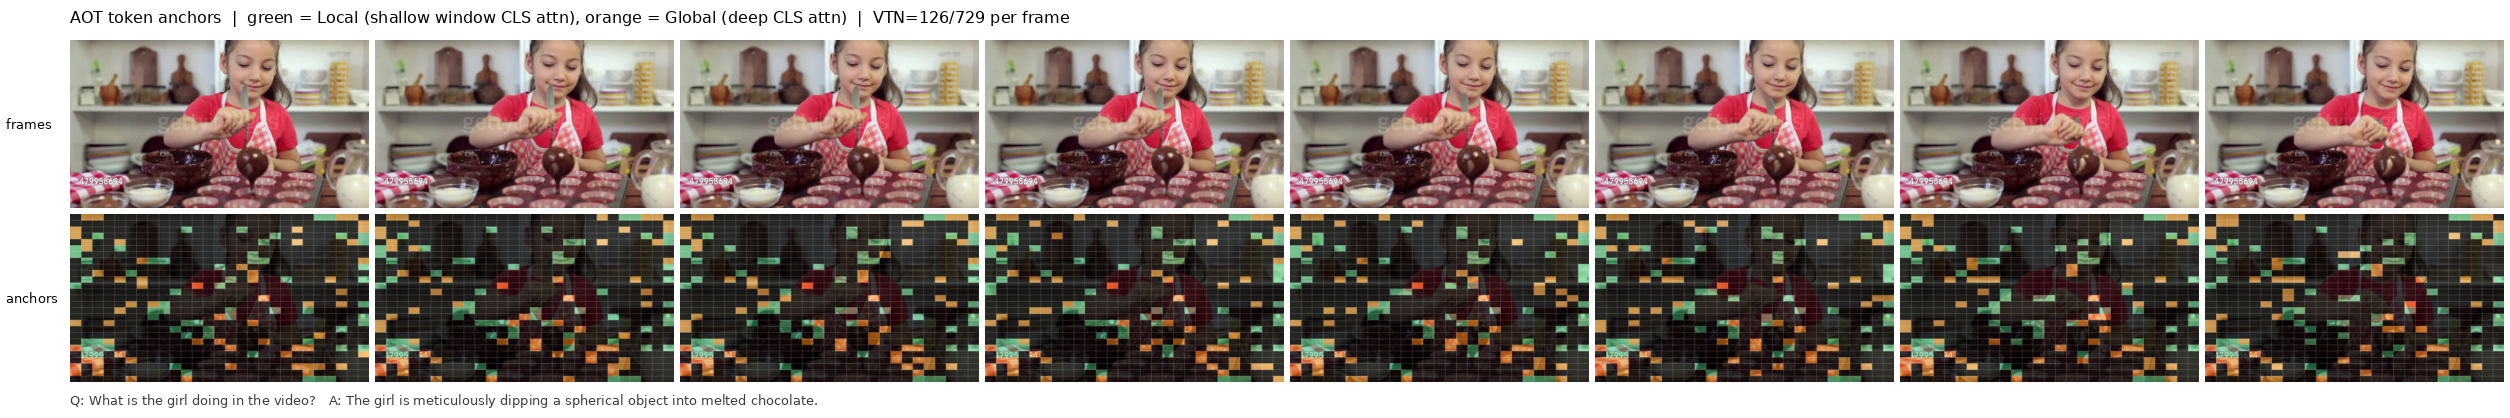
\includegraphics[width=\textwidth]{visualizations/out/aot_anchors_cooking_muffins.png}
\caption{Qualitative visualization of AOT's local/global token anchors on a new cooking video (LLaVA-OV-7B, VTN$=126/729$ per frame), captured from the same instrumented code path as the tables above. Top: sampled frames; bottom: \textcolor[RGB]{30,150,80}{green} = Local anchors (shallow-layer window CLS attention), \textcolor[RGB]{220,120,0}{orange} = Global anchors (deep-layer CLS attention); unselected patches are dimmed and later merged into the anchors via optimal transport. Anchors concentrate on the girl's face, hands, and the chocolate she is dipping. More examples in \texttt{visualizations/out/}.}
\end{figure}

\end{document}
